\documentclass[11pt,a4paper]{article}

\usepackage[T1]{fontenc}
\usepackage[utf8]{inputenc}
\usepackage{lmodern}
\usepackage{microtype}
\usepackage[a4paper,margin=27mm,headheight=14pt]{geometry}
\usepackage{amsmath,amssymb,amsthm,mathtools,bm}
\usepackage{booktabs,tabularx,array,longtable}
\usepackage{enumitem}
\usepackage{xcolor}
\usepackage{graphicx}
\usepackage{tikz}
\usetikzlibrary{arrows.meta,positioning,calc,shapes.geometric,fit}
\usepackage{pgfplots}
\pgfplotsset{compat=1.18}
\usepackage{listings}
\usepackage{fancyhdr}
\usepackage{hyperref}
\usepackage[nameinlink,noabbrev]{cleveref}

\definecolor{noteblue}{RGB}{25,68,120}
\definecolor{notegreen}{RGB}{35,110,75}
\definecolor{notered}{RGB}{150,45,45}
\definecolor{notegray}{RGB}{75,82,90}
\definecolor{lightblue}{RGB}{236,244,252}
\definecolor{lightgreen}{RGB}{237,248,241}
\definecolor{lightred}{RGB}{252,240,240}
\definecolor{lightgray}{RGB}{246,247,248}

\hypersetup{
  colorlinks=true,
  linkcolor=noteblue,
  citecolor=notegreen,
  urlcolor=noteblue,
  pdftitle={Zero-Level-Set-Preserving Source Terms for Gradient Control in Level-Set Transport},
  pdfsubject={Technical note on combined normal-strain cancellation and gradient relaxation},
  pdfkeywords={level set, signed distance, curvature, source term, SDPLS, parasitic currents, reinitialization}
}

\pagestyle{fancy}
\fancyhf{}
\fancyhead[L]{\small Combined source terms for level-set gradient control}
\fancyhead[R]{\small Technical note}
\fancyfoot[C]{\thepage}

\setlength{\parindent}{0pt}
\setlength{\parskip}{0.55em}
\setlist[itemize]{leftmargin=1.5em,itemsep=0.25em,topsep=0.25em}
\setlist[enumerate]{leftmargin=1.7em,itemsep=0.25em,topsep=0.25em}
\allowdisplaybreaks

\newtheorem{theorem}{Theorem}[section]
\newtheorem{proposition}[theorem]{Proposition}
\newtheorem{lemma}[theorem]{Lemma}
\newtheorem{corollary}[theorem]{Corollary}
\theoremstyle{definition}
\newtheorem{definition}[theorem]{Definition}
\newtheorem{assumption}[theorem]{Assumption}
\theoremstyle{remark}
\newtheorem{remark}[theorem]{Remark}

\newcommand{\R}{\mathbb{R}}
\newcommand{\dt}{\partial_t}
\newcommand{\D}{\mathrm{D}}
\newcommand{\Div}{\operatorname{div}}
\newcommand{\tr}{\operatorname{tr}}
\newcommand{\dist}{\operatorname{dist}}
\newcommand{\sign}{\operatorname{sign}}
\newcommand{\supp}{\operatorname{supp}}
\newcommand{\Id}{\mathrm{I}}
\newcommand{\sym}{\operatorname{sym}}
\newcommand{\jump}[1]{\llbracket #1 \rrbracket}
\newcommand{\norm}[1]{\left\lVert #1\right\rVert}
\newcommand{\abs}[1]{\left\lvert #1\right\rvert}
\newcommand{\inner}[2]{\left\langle #1,#2\right\rangle}
\newcommand{\material}{\mathrm{D}_t}
\newcommand{\SigmaT}{\Sigma(t)}
\newcommand{\ph}{\phi_h}
\newcommand{\vh}{v_h}
\newcommand{\gh}{g_h}
\newcommand{\nh}{n_h}
\newcommand{\ah}{a_h}
\newcommand{\ahat}{\widehat a_h}

\newenvironment{keybox}[1]{%
  \begin{center}\begin{minipage}{0.94\textwidth}
  \color{noteblue}\hrule\vspace{0.5em}
  \textbf{#1}\par\color{black}\vspace{0.3em}
}{%
  \vspace{0.4em}\color{noteblue}\hrule\color{black}
  \end{minipage}\end{center}
}

\lstdefinestyle{pseudocode}{
  basicstyle=\ttfamily\small,
  keywordstyle=\bfseries\color{noteblue},
  commentstyle=\itshape\color{notegray},
  columns=fullflexible,
  frame=single,
  rulecolor=\color{notegray},
  backgroundcolor=\color{lightgray},
  xleftmargin=0.5em,
  xrightmargin=0.5em,
  aboveskip=0.8em,
  belowskip=0.8em,
  breaklines=true,
  showstringspaces=false
}

\title{\vspace{-1.5cm}\textbf{Zero-Level-Set-Preserving Source Terms for Gradient Control in Level-Set Transport}\\[0.5em]
\large Analysis, design, and implementation of a combined normal-strain cancellation and relaxation approach}
\author{Technical note for scientific discussion and numerical implementation}
\date{6 August 2026}

\begin{document}
\maketitle

\begin{abstract}
A level-set function is geometrically redundant: only its zero level represents the physical interface, while its values away from the interface may be modified to improve numerical conditioning. This note develops that observation into a detailed analysis of source terms of the form
\[
  \partial_t\phi+v\cdot\nabla\phi=\phi F,
\]
which vanish on the zero level and therefore preserve the continuum interface motion. The focus is a combined source
\[
  F=a+\lambda(1-\abs{\nabla\phi}),
  \qquad
  a=n^{\mathsf T}D(v)n,
  \qquad
  n=\frac{\nabla\phi}{\abs{\nabla\phi}},
\]
where the normal strain $a$ cancels the deformation of the gradient caused by advection, while the relaxation term drives the interfacial gradient magnitude toward one. On the exact interface the resulting evolution is the logistic equation
\[
  \material \abs{\nabla\phi}=\lambda\abs{\nabla\phi}\bigl(1-\abs{\nabla\phi}\bigr),
\]
independent of the velocity-gradient norm. The note derives this identity and its perturbation under approximate, filtered, or discretely inconsistent strain cancellation; analyzes narrow-band localization and curvature conditioning; proposes finite-volume and finite-element implementation patterns; identifies failure modes associated with parasitic currents; and presents a verification matrix and diagnostics. A discrete multiplicative-corrector variant is also developed as an alternative that estimates and cancels the actual gradient deformation produced by the advection update, avoiding an explicit velocity-gradient evaluation. Established results from the locally signed-distance-preserving level-set method, the mathematical analysis of modified level-set equations, and the velocity-extension method are separated from the new synthesis and implementation recommendations proposed here.
\end{abstract}

\begin{keybox}{Status of the material}
The geometric identities and the general equation $\material\phi=\phi F$ are standard. The choice $F=a$ is the SDPLS source of Fricke et al.\ \cite{FrickeEtAl2022}; rigorous well-posedness results for that class and a simpler source $F=\beta-\abs{\nabla\phi}$ are given by Bothe, Fricke, and Soga \cite{BotheFrickeSoga2024}; the velocity-extension method is analyzed by Bothe and Soga \cite{BotheSoga2026}. The combined source $F=a+\lambda(1-g)$, its residual-cancellation analysis, and the discrete multiplicative-corrector strategy are presented here as a synthesis and as proposals for investigation, not as claims that they already appear in those references.
\end{keybox}

\tableofcontents
\newpage

\section{Scope and principal conclusions}

Let $\Sigma(t)\subset\Omega\subset\R^d$ be a sufficiently smooth moving hypersurface represented as
\[
  \Sigma(t)=\{x\in\Omega:\phi(t,x)=0\},
  \qquad \nabla\phi\neq0\quad\text{on }\Sigma(t).
\]
The physical geometry is invariant under any smooth change of defining function that preserves the regular zero level and its orientation. Numerically, however, normals and curvature are computed from derivatives of $\phi$ in a stencil around the interface. The off-interface representation therefore has no direct physical meaning but has a decisive conditioning role.

The central proposal is the narrow-band equation
\begin{equation}
  \partial_t\phi+v\cdot\nabla\phi
  =\chi\!\left(\frac{\phi}{\varepsilon_b}\right)\phi
  \left[\widehat a+\lambda\left(1-g\right)\right],
  \qquad
  g=\abs{\nabla\phi},
  \label{eq:main-discrete-continuous}
\end{equation}
where $\chi(0)=1$, $\lambda>0$, and $\widehat a$ approximates
\begin{equation}
  a=n^{\mathsf T}\nabla v\,n=n^{\mathsf T}D(v)n,
  \qquad
  D(v)=\frac12\left(\nabla v+\nabla v^{\mathsf T}\right).
  \label{eq:normal-strain}
\end{equation}
The antisymmetric part of $\nabla v$ drops out, hence $a$ is the normal normal component of the rate-of-deformation tensor.

The main conclusions are:
\begin{enumerate}
  \item The factor $\phi$ preserves the zero level at the continuum level, provided the coefficient is regular enough along characteristics.
  \item With exact cancellation $\widehat a=a$, the interfacial gradient magnitude satisfies a velocity-independent logistic equation and converges to one from every positive initial value.
  \item With cancellation error $\delta=\widehat a-a$, the relevant stability quantity is $\delta$, not $\norm{\nabla v}_{\infty}$. If $\abs\delta\le\eta<\lambda$, the interval $[1-\eta/\lambda,1+\eta/\lambda]$ is invariant.
  \item Large parasitic velocity gradients are not automatically harmless. They are harmless only to the extent that their effect on gradient transport is cancelled consistently. A noisy or filtered $\widehat a$ may leave a large residual $\delta$.
  \item A flat-core narrow-band cutoff preserves the exact interfacial law; away from the interface there are $O(\abs\phi)$ perturbations and cutoff-transition terms.
  \item For implementation, positivity-preserving source integration, consistent derivative reconstruction, and diagnostics for the cancellation residual are more important than formally high-order formulas in isolation.
  \item A predictor--corrector multiplication can cancel the actual discrete gradient change after the advection step without explicitly differentiating $v$. This deserves separate numerical study because projection back into a discrete function space can move the discrete zero contour.
\end{enumerate}

\section{Geometric setting}

\subsection{Tubular coordinates and signed distance}

Assume that, over the time interval of interest, $\Sigma(t)$ admits a tubular neighborhood $U_{\rho}(t)$ in which the metric projection $p_t$ is single-valued and smooth. Let $n_t$ be a chosen unit normal on $\Sigma(t)$. Every $x\in U_\rho(t)$ has the unique representation
\begin{equation}
  x=p_t(x)+d(t,x)n_t(p_t(x)),
  \label{eq:tubular-decomp}
\end{equation}
where $d$ is the signed distance. Consequently,
\begin{equation}
  d(t,x)=\inner{x-p_t(x)}{n_t(p_t(x))},
  \qquad
  \nabla d(t,x)=n_t(p_t(x)),
  \qquad
  \abs{\nabla d}=1.
\end{equation}
If the surface is transported by a smooth velocity field $v$, then for fixed $x$ in the tubular neighborhood,
\begin{equation}
  \partial_t d(t,x)=-v(t,p_t(x))\cdot n_t(p_t(x)).
  \label{eq:distance-time}
\end{equation}
Equivalently, the signed distance satisfies a transport equation with the normal extension of the interface velocity,
\begin{equation}
  \partial_t d+\widetilde v\cdot\nabla d=0,
  \qquad
  \widetilde v(t,x)=v(t,p_t(x)).
  \label{eq:extended-velocity-distance}
\end{equation}
This is the geometric basis of the velocity-extension method \cite{BotheSoga2026}.

\subsection{Normal and curvature from a general defining function}

For a regular level-set function that is not a signed distance,
\begin{equation}
  n=\frac{\nabla\phi}{\abs{\nabla\phi}},
  \qquad
  P=\Id-n\otimes n.
\end{equation}
The total curvature, with sign determined by the normal convention, is
\begin{equation}
  \kappa=\Div n
  =\Div\left(\frac{\nabla\phi}{\abs{\nabla\phi}}\right)
  =\frac{1}{\abs{\nabla\phi}}P:D^2\phi.
  \label{eq:curvature-general}
\end{equation}
In expanded form,
\begin{equation}
  \kappa
  =\frac{\abs{\nabla\phi}^2\Delta\phi
  -\nabla\phi^{\mathsf T}D^2\phi\,\nabla\phi}
  {\abs{\nabla\phi}^3}.
  \label{eq:curvature-expanded}
\end{equation}
For a signed distance, $\kappa=\Delta d$ on the interface. Formula \eqref{eq:curvature-expanded} makes the conditioning problem explicit: derivative errors are amplified when $g=\abs{\nabla\phi}$ becomes small, even though exact curvature is invariant under positive rescaling of a smooth defining function.

\subsection{Why off-interface modification can improve on-interface curvature}

If $\widetilde\phi=a(x)\phi$ with $a>0$ near the interface, then
\[
  \nabla\widetilde\phi=a\nabla\phi\quad\text{on }\Sigma(t),
\]
so the exact normal and curvature are unchanged. A finite-difference, finite-volume, or finite-element curvature evaluation uses neighboring values and reconstructed derivatives; therefore the choice of $a$ away from the interface affects truncation error, noise amplification, and stencil robustness. The useful objective is not to assign physical significance to $\phi$ away from zero, but to construct a smooth, well-resolved defining function with $g$ bounded away from zero and preferably close to one in the curvature stencil.

\section{Gradient deformation under standard advection}

Let
\begin{equation}
  \material:=\partial_t+v\cdot\nabla,
  \qquad
  q:=\nabla\phi,
  \qquad
  g:=\abs q,
  \qquad
  n:=q/g.
\end{equation}
For the standard level-set equation
\begin{equation}
  \material\phi=0,
  \label{eq:standard-advection}
\end{equation}
spatial differentiation gives
\begin{equation}
  \material q=-(\nabla v)^{\mathsf T}q.
  \label{eq:q-standard}
\end{equation}
Taking the scalar product with $n$ yields
\begin{equation}
  \material g=-g\,a,
  \qquad
  a:=n^{\mathsf T}(\nabla v)n=n^{\mathsf T}D(v)n.
  \label{eq:g-standard}
\end{equation}
Hence
\begin{equation}
  \material\log g=-a.
  \label{eq:logg-standard}
\end{equation}
Along a material trajectory $X(t)$ on the interface,
\begin{equation}
  g(t,X(t))=g(0,X(0))
  \exp\left(-\int_0^t a(s,X(s))\,\mathrm ds\right).
  \label{eq:g-standard-exact}
\end{equation}
A signed-distance initial condition is therefore not preserved unless the accumulated normal strain vanishes.

The unit normal satisfies
\begin{equation}
  \material n=-P(\nabla v)^{\mathsf T}n.
  \label{eq:normal-evolution}
\end{equation}
This is the geometric rotation law for a material normal. The scalar $a$ controls the magnitude of the level-set gradient; the tangential projection controls the direction.

\subsection{Relation to interface area generation}

The surface divergence is
\begin{equation}
  \Div_{\Sigma}v=P:\nabla v=\Div v-a.
\end{equation}
For incompressible flow, $\Div v=0$, so
\begin{equation}
  a=-\Div_{\Sigma}v.
\end{equation}
Thus $-a$ is the local material rate of interfacial area generation, which is the interpretation used in the SDPLS construction \cite{FrickeEtAl2022}.

\section{General zero-level-preserving source terms}

Consider
\begin{equation}
  \material\phi=\phi F(t,x,\phi,\nabla\phi).
  \label{eq:general-source}
\end{equation}
The following elementary observation is the basis for all source terms considered here.

\begin{proposition}[Continuum zero-set and sign preservation]
Assume $F$ is integrable along the characteristics of $v$. If $X$ solves $\dot X=v(t,X)$, then
\begin{equation}
  \phi(t,X(t))=\phi(0,X(0))
  \exp\left(\int_0^t F(s,X(s),\phi,\nabla\phi)\,\mathrm ds\right).
  \label{eq:char-solution}
\end{equation}
Consequently, zero values remain zero and nonzero values retain their sign.
\end{proposition}

\begin{remark}
The proposition is a continuum statement. A discrete update followed by interpolation, projection, limiting, or remeshing can move the numerical zero contour even when the continuous source is proportional to $\phi$.
\end{remark}

Differentiating \eqref{eq:general-source} gives
\begin{equation}
  \material q=-(\nabla v)^{\mathsf T}q+Fq+\phi\nabla F.
  \label{eq:q-general}
\end{equation}
Therefore
\begin{equation}
  \boxed{
  \material g=g(F-a)+\phi\,\partial_nF,
  }
  \qquad
  \partial_nF:=n\cdot\nabla F.
  \label{eq:g-general}
\end{equation}
On the interface,
\begin{equation}
  \boxed{
  \material^{\Sigma} g=g(F-a),
  }
  \label{eq:g-interface-general}
\end{equation}
where $\material^{\Sigma}$ denotes differentiation along an interfacial material trajectory. The normal evolution is
\begin{equation}
  \material n=-P(\nabla v)^{\mathsf T}n+\frac{\phi}{g}P\nabla F,
  \label{eq:n-general}
\end{equation}
so on $\Sigma(t)$ the source has no direct effect on the normal direction:
\begin{equation}
  \material^{\Sigma}n=-P(\nabla v)^{\mathsf T}n.
  \label{eq:n-interface}
\end{equation}
This is another expression of geometric invariance: the source changes the parameterization of the defining function, not the interface geometry.

\section{Existing strategies and their relation}

\subsection{SDPLS: exact preservation of the interfacial gradient magnitude}

The SDPLS choice is
\begin{equation}
  F=a=n^{\mathsf T}(\nabla v)n.
  \label{eq:sdpls-source}
\end{equation}
Then \eqref{eq:g-interface-general} gives
\begin{equation}
  \material^{\Sigma}g=0.
  \label{eq:sdpls-preservation}
\end{equation}
If $g=1$ initially on the interface, it remains one there. Off the interface,
\begin{equation}
  \material g=\phi\,\partial_n a,
  \label{eq:sdpls-off-interface}
\end{equation}
up to the sign convention used to define the rate $\mathcal R=-a$ in \cite{FrickeEtAl2022}. Thus SDPLS is exactly local at the interface; it does not generally generate the signed-distance property throughout a tubular neighborhood.

\subsection{Simpler nonlinear source}

Bothe, Fricke, and Soga also analyze the source
\begin{equation}
  F=\beta-g,
  \qquad \beta>0,
  \label{eq:simple-source}
\end{equation}
which gives on the interface
\begin{equation}
  \material^{\Sigma}g=g(\beta-g-a).
  \label{eq:simple-g}
\end{equation}
If $\abs a\le\alpha<\beta$, then
\begin{equation}
  \beta-\alpha\le g\le\beta+\alpha
  \label{eq:simple-invariant}
\end{equation}
is an invariant interval for the interfacial ODE. The rigorous analysis in \cite{BotheFrickeSoga2024} establishes smooth local-in-space solutions and an a priori gradient bound in a tubular neighborhood under appropriate regularity assumptions.

The drawback for two-phase-flow computation is structural: the parameter $\beta$ must dominate a normal-strain bound. A grid-scale parasitic velocity of amplitude $U_p$ and wavelength $O(h)$ can produce
\begin{equation}
  \norm{\nabla v_h}_{\infty}=O(U_p/h),
  \label{eq:parasitic-scaling}
\end{equation}
which may grow under refinement even if $U_p$ is small. A parameter chosen from a global norm can then become stiff, mesh-dependent, and controlled by a localized numerical defect.

\subsection{Velocity extension}

The velocity-extension method uses
\begin{equation}
  \widetilde v(t,x)=v(t,p_t(x))
\end{equation}
and transports the level set with $\widetilde v$. If the initial level set is the local signed distance, the method produces the local signed distance of the moving interface in a tubular neighborhood. Bothe and Soga give a rigorous formulation and global-in-time/local-in-space smooth well-posedness, as well as global viscosity solutions \cite{BotheSoga2026}. In fully nonlinear form, one of the corresponding equations is
\begin{equation}
  \partial_t\phi+
  v\!\left(t,x-\phi\frac{\nabla\phi}{\abs{\nabla\phi}^2}\right)\cdot\nabla\phi=0.
  \label{eq:velocity-extension-nonlinear}
\end{equation}
Velocity extension controls $g$ in a neighborhood, rather than only on the interface, but requires a geometric extension or an equivalent nonlinear transport operator.

\begin{table}[htbp]
\centering
\caption{Comparison of gradient-control mechanisms.}
\label{tab:comparison}
\small
\begin{tabularx}{\textwidth}{@{}p{0.19\textwidth}p{0.24\textwidth}X X@{}}
\toprule
Method & Governing modification & Exact continuum property & Principal implementation issue \\
\midrule
Standard advection & $\material\phi=0$ & Correct zero-level motion & $g$ is exponentially stretched by $a$ \\
SDPLS & $\material\phi=\phi a$ & $\material^\Sigma g=0$ & Requires $n^{\mathsf T}\nabla v\,n$ \\
Simpler source & $\material\phi=\phi(\beta-g)$ & A priori bounds under $\beta>\alpha$ & Parameter depends on strain bound \\
Combined source & $\material\phi=\phi[a+\lambda(1-g)]$ & $\material^\Sigma g=\lambda g(1-g)$ & Requires accurate cancellation or residual control \\
Velocity extension & $\partial_t\phi+\widetilde v\cdot\nabla\phi=0$ & Signed-distance structure in a tube & Projection/extension and nonlinear transport \\
Reinitialization & Pseudo-time eikonal correction & Restores $g\approx1$ & Interface drift and contact-line treatment \\
\bottomrule
\end{tabularx}
\end{table}

\section{Combined normal-strain cancellation and relaxation}

\subsection{Definition}

The proposed combined coefficient is
\begin{equation}
  F=a+\lambda(1-g),
  \qquad \lambda>0.
  \label{eq:combined-F}
\end{equation}
The full equation is
\begin{equation}
  \boxed{
  \partial_t\phi+v\cdot\nabla\phi
  =\phi\left[n^{\mathsf T}D(v)n+\lambda\left(1-\abs{\nabla\phi}\right)\right].
  }
  \label{eq:combined-PDE}
\end{equation}
The first term cancels the physical deformation of $g$ generated by advection; the second corrects pre-existing or numerically generated deviations from the signed-distance scaling.

\begin{figure}[htbp]
\centering
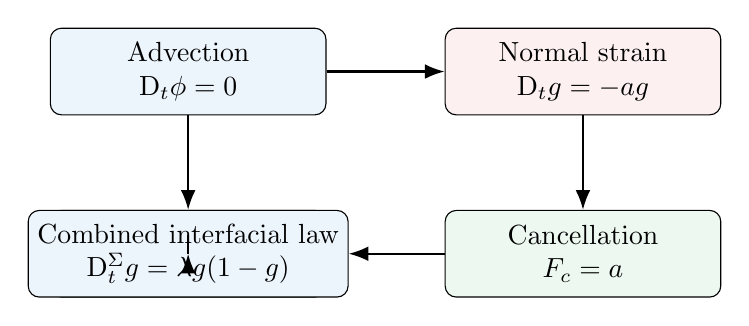
\begin{tikzpicture}[
  node distance=12mm and 15mm,
  box/.style={draw,rounded corners,align=center,minimum height=11mm,minimum width=35mm,fill=lightblue},
  gbox/.style={draw,rounded corners,align=center,minimum height=11mm,minimum width=35mm,fill=lightgreen},
  rbox/.style={draw,rounded corners,align=center,minimum height=11mm,minimum width=35mm,fill=lightred},
  arr/.style={-{Latex[length=2.5mm]},thick}
]
\node[box] (adv) {Advection\\$\material\phi=0$};
\node[rbox,right=of adv] (strain) {Normal strain\\$\material g=-ag$};
\node[gbox,below=of strain] (cancel) {Cancellation\\$F_c=a$};
\node[gbox,left=of cancel] (relax) {Relaxation\\$F_r=\lambda(1-g)$};
\node[box,below=of adv] (result) {Combined interfacial law\\$\material^\Sigma g=\lambda g(1-g)$};
\draw[arr] (adv)--(strain);
\draw[arr] (strain)--(cancel);
\draw[arr] (cancel)--(result);
\draw[arr] (relax)--(result);
\draw[arr] (adv)--(result);
\end{tikzpicture}
\caption{Decomposition of the combined source. The cancellation term removes the normal-strain contribution; the remaining interfacial dynamics is a controlled relaxation.}
\label{fig:combined-flow}
\end{figure}

\subsection{Exact interfacial law}

Substitution of \eqref{eq:combined-F} into \eqref{eq:g-interface-general} yields
\begin{equation}
  \boxed{
  \material^{\Sigma}g=\lambda g(1-g).
  }
  \label{eq:logistic}
\end{equation}
No norm of $\nabla v$ appears. For constant $\lambda$, the solution along an interfacial trajectory is
\begin{equation}
  \boxed{
  g(t)=\frac{1}{1+\left(g_0^{-1}-1\right)e^{-\lambda t}}.
  }
  \label{eq:logistic-solution}
\end{equation}
For $g_0>0$,
\begin{equation}
  \min\{g_0,1\}\le g(t)\le\max\{g_0,1\},
  \qquad
  g(t)\to1.
\end{equation}
If $g_0=1$, then $g\equiv1$. If $g_0=0$, the equation cannot regenerate regularity; $g=0$ remains an equilibrium.

For variable $\lambda(t,X(t))\ge0$, define
\[
  \Lambda(t)=\int_0^t\lambda(s,X(s))\,\mathrm ds.
\]
Then
\begin{equation}
  g(t)=\frac{1}{1+\left(g_0^{-1}-1\right)e^{-\Lambda(t)}}.
\end{equation}
Convergence follows if $\Lambda(t)\to\infty$.

\begin{figure}[htbp]
\centering
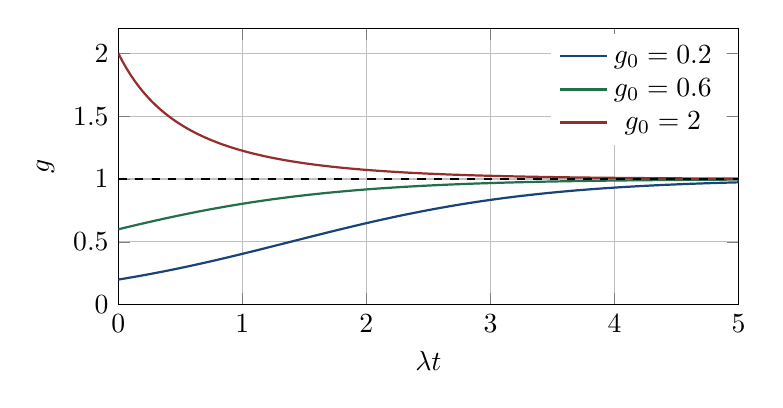
\begin{tikzpicture}
\begin{axis}[
  width=0.78\textwidth,
  height=0.42\textwidth,
  xlabel={$\lambda t$},
  ylabel={$g$},
  xmin=0,xmax=5,
  ymin=0,ymax=2.2,
  grid=major,
  legend style={at={(0.98,0.98)},anchor=north east,draw=none,fill=white},
  samples=150
]
\addplot[thick,noteblue,domain=0:5] {1/(1+(1/0.2-1)*exp(-x))};
\addlegendentry{$g_0=0.2$}
\addplot[thick,notegreen,domain=0:5] {1/(1+(1/0.6-1)*exp(-x))};
\addlegendentry{$g_0=0.6$}
\addplot[thick,notered,domain=0:5] {1/(1+(1/2-1)*exp(-x))};
\addlegendentry{$g_0=2$}
\addplot[dashed,black,domain=0:5] {1};
\end{axis}
\end{tikzpicture}
\caption{Exact logistic relaxation of the interfacial gradient magnitude under the combined source.}
\label{fig:logistic}
\end{figure}

\subsection{Linearization and relaxation time}

Let $e=g-1$. Then
\begin{equation}
  \material^{\Sigma}e=-\lambda e-\lambda e^2.
\end{equation}
For small errors,
\begin{equation}
  \material^{\Sigma}e\approx-\lambda e,
\end{equation}
so the relaxation time is
\begin{equation}
  \tau_r=\lambda^{-1}.
  \label{eq:relaxation-time}
\end{equation}
The parameter should therefore be chosen from the desired physical or numerical correction timescale, rather than from a global velocity-gradient maximum.

\subsection{General target and feedback law}

A target $g_*>0$ can be imposed by
\begin{equation}
  F=a+\lambda(g_*-g),
\end{equation}
which gives
\begin{equation}
  \material^{\Sigma}g=\lambda g(g_*-g).
\end{equation}
The signed-distance target corresponds to $g_*=1$. More generally, a source
\begin{equation}
  F=a+\Psi(g)
\end{equation}
produces
\begin{equation}
  \material^{\Sigma}g=g\Psi(g).
\end{equation}
To obtain linear relaxation $\material^{\Sigma}g=-\lambda(g-1)$ one would require
\begin{equation}
  \Psi(g)=\lambda\left(\frac1g-1\right),
\end{equation}
which is singular as $g\to0$. The logistic choice is smooth for $g\ge0$ and preserves positivity, at the price of slower absolute recovery when $g\ll1$.

\section{Approximate cancellation and robustness}

\subsection{Residual-cancellation equation}

In computation, replace $a$ by $\widehat a$. Define
\begin{equation}
  \delta:=\widehat a-a.
  \label{eq:delta}
\end{equation}
Then the interfacial equation becomes
\begin{equation}
  \boxed{
  \material^{\Sigma}g=g\left[\lambda(1-g)+\delta\right].
  }
  \label{eq:perturbed-logistic}
\end{equation}
The key robustness quantity is the residual $\delta$, which includes:
\begin{itemize}
  \item truncation error in $\nabla v$ and $n$;
  \item interpolation mismatch between velocity and level-set grids;
  \item filtering or clipping of the strain;
  \item temporal lagging of $a$;
  \item inconsistency between the continuous strain formula and the actual discrete deformation produced by the advection operator;
  \item projection and reconstruction errors.
\end{itemize}

\begin{proposition}[Invariant residual tube]
Assume $\abs{\delta}\le\eta<\lambda$ on the interface. Then
\begin{equation}
  I_\eta=\left[1-\frac{\eta}{\lambda},\,1+\frac{\eta}{\lambda}\right]
  \label{eq:residual-tube}
\end{equation}
is invariant for \eqref{eq:perturbed-logistic}. Solutions with $g_0>0$ outside $I_\eta$ are driven toward it.
\end{proposition}

\begin{proof}
At the lower endpoint, the bracket in \eqref{eq:perturbed-logistic} is $\eta+\delta\ge0$; at the upper endpoint it is $-\eta+\delta\le0$. Outside the interval the sign points inward.
\end{proof}

For constant $\delta$, the positive equilibrium is
\begin{equation}
  g_*=1+\frac{\delta}{\lambda},
  \label{eq:constant-delta-equilibrium}
\end{equation}
provided $\delta> -\lambda$.

\subsection{Reciprocal-gradient representation}

With $z=1/g$, \eqref{eq:perturbed-logistic} becomes the linear equation
\begin{equation}
  \material^{\Sigma}z=-(\lambda+\delta)z+\lambda.
  \label{eq:z-linear}
\end{equation}
This representation is useful for analysis and diagnostics. It shows explicitly that a sufficiently negative residual, $\delta\le-\lambda$, destroys attraction to a positive equilibrium. It also gives the variation-of-constants formula
\begin{equation}
  z(t)=e^{-A(t)}z_0+\int_0^t e^{-[A(t)-A(s)]}\lambda(s)\,\mathrm ds,
  \qquad
  A(t)=\int_0^t(\lambda+\delta)\,\mathrm ds.
\end{equation}

\subsection{Small-signal response to cancellation noise}

For $g=1+e$ with small $e$ and $\delta$,
\begin{equation}
  \dot e+\lambda e\approx\delta.
  \label{eq:linear-noise}
\end{equation}
For a harmonic residual $\delta=\Re(\delta_0e^{i\omega t})$, the response amplitude is
\begin{equation}
  \abs{e_0}=\frac{\abs{\delta_0}}{\sqrt{\lambda^2+\omega^2}}.
\end{equation}
Thus $\lambda$ reduces low-frequency bias and sets the correction bandwidth. High-frequency residuals are attenuated by the gradient dynamics, but they may still contaminate the source update and neighboring derivatives before this asymptotic response is realized.

\subsection{Parasitic currents and large velocity gradients}

A typical capillary computation can develop a feedback loop:
\begin{equation}
  \begin{aligned}
  \text{curvature error}
  &\longrightarrow \text{surface-force imbalance}
  \longrightarrow \text{parasitic }v_h\longrightarrow \nabla v_h,\\
  &\longrightarrow \text{deformation of }g_h
  \longrightarrow \text{larger curvature error}.
  \end{aligned}
\end{equation}
The combined source can break the $\nabla v_h\to g_h$ link only if $\widehat a_h$ reproduces the effective normal strain acting through the discrete advection update. A large $a_h$ is not itself fatal; a large mismatch $\delta_h$ is.

This distinction suggests reporting both
\begin{equation}
  A_h(t)=\norm{a_h}_{L^\infty(\Sigma_h)},
  \qquad
  \Delta_h(t)=\norm{\widehat a_h-a_h^{\mathrm{eff}}}_{L^\infty(\Sigma_h)},
  \label{eq:diagnostic-strains}
\end{equation}
where $a_h^{\mathrm{eff}}$ is an estimate of the gradient deformation actually generated by the advection scheme. The latter quantity is more predictive of gradient-control failure.

\section{Off-interface dynamics and narrow-band localization}

\subsection{Full-band equation}

For $F=a+\lambda(1-g)$, \eqref{eq:g-general} gives
\begin{equation}
  \material g
  =\lambda g(1-g)+\phi\,\partial_n\left[a+\lambda(1-g)\right].
  \label{eq:off-interface-combined}
\end{equation}
The desired logistic law is exact on $\phi=0$. In a sufficiently smooth tube,
\begin{equation}
  \material g=\lambda g(1-g)+O(\abs\phi)
  \label{eq:off-interface-Ophi}
\end{equation}
provided the normal derivative of the coefficient is bounded. This gives local, not global, signed-distance control.

\subsection{Cutoff with a flat core}

Let
\begin{equation}
  F=\chi(\phi/\varepsilon_b)B,
  \qquad
  B=\widehat a+\lambda(1-g),
  \label{eq:cutoff-F}
\end{equation}
with $\chi(0)=1$. Then
\begin{align}
  \material g
  ={}&g\left[-a+\chi B\right]
  +\phi\chi\,\partial_nB
  +\frac{\phi g}{\varepsilon_b}\chi'\!\left(\frac{\phi}{\varepsilon_b}\right)B.
  \label{eq:cutoff-g}
\end{align}
The interfacial law is unchanged. A recommended cutoff has a flat core:
\begin{equation}
  \chi(s)=1\quad\text{for }\abs s\le c_1,
  \qquad
  \chi(s)=0\quad\text{for }\abs s\ge c_2,
  \qquad 0<c_1<c_2.
\end{equation}
In the core, the cutoff derivative vanishes. The transition zone is not expected to retain signed-distance quality; it only decouples the source from the far field.

\begin{keybox}{Practical narrow-band objective}
The objective should be $g\approx1$ in the cells used for normal and curvature reconstruction. It is unnecessary, and often counterproductive, to enforce signed-distance behavior over the whole computational domain.
\end{keybox}

\subsection{Regularization of the normal}

A numerical normal is often defined by
\begin{equation}
  n_\epsilon=\frac{\nabla\phi}{\sqrt{\abs{\nabla\phi}^2+\epsilon_n^2}}.
  \label{eq:regularized-normal}
\end{equation}
This prevents division by zero but changes both the curvature and the strain coefficient. In the active band, $\epsilon_n$ should be small compared with the target gradient scale, which is one in dimensional signed-distance units. A useful diagnostic is the fraction of curvature-stencil points for which $g_h\le c\epsilon_n$; if this fraction is non-negligible, regularization is masking a loss of level-set regularity rather than merely protecting the computation.

\section{Discrete design principles}

\subsection{Separate the continuum model from the discrete mechanism}

At the continuum level, the combined model is unambiguous. At the discrete level, three different objects must be distinguished:
\begin{enumerate}
  \item the strain $a_h^{\mathrm{geom}}=n_h^{\mathsf T}D_h(v_h)n_h$ computed from reconstructed fields;
  \item the effective strain $a_h^{\mathrm{eff}}$ that describes how the chosen advection update changes $g_h$;
  \item the source coefficient $\widehat a_h$ actually inserted in the scheme.
\end{enumerate}
Even if $a_h^{\mathrm{geom}}$ is a high-order approximation to $a$, it may fail to cancel $a_h^{\mathrm{eff}}$ because the discrete gradient does not obey the exact product and commutator identities used in deriving \eqref{eq:g-standard}.

\subsection{Direct-gradient implementation}

A direct implementation of \eqref{eq:main-discrete-continuous} proceeds as follows:
\begin{enumerate}
  \item Reconstruct $q_h=\nabla_h\phi_h$ in the active band.
  \item Compute $g_h=\abs{q_h}$ and $n_h=q_h/\max(g_h,\epsilon_n)$.
  \item Reconstruct $D_h(v_h)$ at the same locations and with an interpolation consistent with the velocity used in the level-set flux.
  \item Form $a_h=n_h^{\mathsf T}D_h(v_h)n_h$.
  \item Optionally filter $a_h$ tangentially on the interface and extend it approximately constantly along normals, producing $\widehat a_h$.
  \item Evaluate $S_h=\chi_h\phi_h[\widehat a_h+\lambda(1-g_h)]$.
  \item Advance advection and source with a time integrator that preserves sign in the source substep.
\end{enumerate}

\subsection{Filtering and normal extension}

Filtering $D_h(v_h)$ componentwise in the volume can smear physical strain and mix tangential and normal structures. A more geometric sequence is:
\begin{enumerate}
  \item evaluate $a_h$ on a reconstructed interface or in cut cells;
  \item apply a surface or tangential filter to $a_h$;
  \item extend the scalar coefficient along approximate normals into the active band.
\end{enumerate}
This preserves the meaning of the quantity being filtered and minimizes normal derivatives in \eqref{eq:off-interface-combined}. The filter width should be reported in units of local mesh size and tested for mesh dependence.

\subsection{Time integration of the source}

If the coefficient $r_h=\widehat a_h+\lambda(1-g_h)$ is frozen over a source substep, then
\begin{equation}
  \partial_t\phi_h=r_h\phi_h
\end{equation}
has the exact pointwise update
\begin{equation}
  \boxed{
  \phi_h^{n+1}=e^{\Delta t r_h^n}\phi_h^*.
  }
  \label{eq:exponential-source}
\end{equation}
This preserves the sign of the stored value for any $\Delta t r_h^n$. By contrast, forward Euler,
\begin{equation}
  \phi_h^{n+1}=(1+\Delta t r_h^n)\phi_h^*,
\end{equation}
can reverse signs when $1+\Delta t r_h^n<0$ and create spurious zero crossings.

The exponential update does not remove the accuracy restriction associated with rapidly varying $r_h$; it only integrates the frozen linear source exactly. A practical resolution criterion is
\begin{equation}
  \Delta t\max_{U_b}\abs{r_h}\lesssim C_r
\end{equation}
with $C_r=O(1)$, unless a higher-order exponential or implicit coupling is used.

\subsection{Operator splitting}

A robust second-order pattern is Strang splitting:
\begin{enumerate}
  \item half source step with frozen or predicted $r_h$;
  \item full advection step;
  \item recompute $q_h,g_h,n_h,\widehat a_h$;
  \item half source step.
\end{enumerate}
Because the source is designed to compensate an advection-induced gradient deformation, recomputation after the advection step is important. A single source evaluation before advection can lag the cancellation by one time step and increase $\delta_h$.

\subsection{Finite-volume form}

For incompressible $v$ and a control volume $K$,
\begin{equation}
  \frac{\mathrm d}{\mathrm dt}\bar\phi_K
  +\frac1{|K|}\sum_{f\subset\partial K}\mathcal F_f(\phi,v)
  =\overline{\phi r}_K.
\end{equation}
A common approximation is
\begin{equation}
  \overline{\phi r}_K\approx\bar\phi_K\bar r_K,
\end{equation}
which supports the exponential cellwise source update. Higher-order reconstructions should evaluate $r$ and $\phi$ at quadrature points; otherwise the source accuracy may remain first-order even when the advective flux is high-order.

\subsection{Continuous and discontinuous finite elements}

For continuous finite elements, a weak form is
\begin{equation}
  (\partial_t\phi_h,w_h)+(v_h\cdot\nabla\phi_h,w_h)
  =(\phi_h r_h,w_h),
\end{equation}
with stabilization as required for transport. Mass lumping makes a positive multiplicative source update straightforward but may reduce accuracy. With a consistent mass matrix, a pointwise exponential factor is not equivalent to the Galerkin source solve.

For discontinuous Galerkin methods, element-local multiplication and local projection are natural, but projection can still change the reconstructed zero contour. An elementwise constant positive factor preserves the local zero set of a polynomial exactly; a spatially varying factor followed by projection generally does not.

\section{A discrete multiplicative-corrector alternative}

\subsection{Motivation}

The direct method computes a velocity gradient and hopes that it cancels the gradient deformation generated by the discrete advection operator. An alternative is to measure that deformation after an advection predictor and correct it directly.

Let
\begin{equation}
  \phi^A=\mathcal A_{\Delta t}(\phi^n;v_h)
\end{equation}
be an advection-only predictor. Compute $g^A$ near the new interface. The combined continuum law says that the desired interfacial gradient after the full step is independent of $a$. If the target is exact signed-distance scaling at every step, set
\begin{equation}
  g^{\mathrm{tar}}=1.
\end{equation}
For finite relaxation, the exact logistic map is
\begin{equation}
  \mathcal G_{\Delta t}(g^n)
  =\frac{1}{1+\left((g^n)^{-1}-1\right)e^{-\lambda\Delta t}}.
  \label{eq:logistic-map}
\end{equation}
A multiplicative corrector
\begin{equation}
  \phi^{n+1}=M\phi^A,
  \qquad M>0,
  \label{eq:multiplicative-corrector}
\end{equation}
satisfies on the exact zero level
\begin{equation}
  \nabla\phi^{n+1}=M\nabla\phi^A,
  \qquad
  g^{n+1}=Mg^A.
\end{equation}
Hence the interface value
\begin{equation}
  M_\Sigma=\frac{g^{\mathrm{tar}}}{g^A}
  \label{eq:M-interface}
\end{equation}
sets the desired gradient magnitude. A positive extension of $M_\Sigma$ into the narrow band preserves the continuum zero set.

\subsection{Equivalent frozen source}

The multiplication \eqref{eq:multiplicative-corrector} is equivalent to a frozen source coefficient
\begin{equation}
  r_{\mathrm{corr}}=\frac1{\Delta t}\log M.
  \label{eq:corrector-source}
\end{equation}
This coefficient implicitly includes the actual physical strain, parasitic-current strain, and truncation-induced strain produced by the advection predictor. It avoids explicit evaluation of $\nabla v$.

\subsection{Challenges}

The method is attractive but not automatically zero-contour preserving in a discrete representation:
\begin{itemize}
  \item multiplying nodal values by a spatially varying positive $M_h$ and then using piecewise-linear interpolation can shift the interpolated zero crossing;
  \item $g^n$ must be transported to the new interface if finite relaxation rather than immediate $g=1$ is desired;
  \item computing $M_\Sigma$ requires a reliable interface gradient after the predictor;
  \item extending and projecting $M$ can introduce oscillations;
  \item repeated multiplicative correction may affect mass conservation through discrete interface shifts.
\end{itemize}

A particularly clean realization may be possible in a cut-cell, discontinuous, or interface-reconstruction framework where the correction is applied to a local analytic defining function while the reconstructed interface is held fixed.

\begin{keybox}{Research hypothesis}
A predictor--multiplicative-corrector method may be more robust to parasitic velocity gradients than direct SDPLS cancellation because it cancels the observed discrete gradient deformation rather than an independently reconstructed $n^{\mathsf T}D(v)n$. Its decisive test is whether the chosen discrete function-space projection preserves the interface more accurately than it improves $g$ and curvature.
\end{keybox}

\section{Recommended implementation workflow}

\subsection{Baseline direct combined method}

\begin{lstlisting}[style=pseudocode,caption={One time step of a direct combined-source level-set update.}]
Given phi^n, velocity v^n, time step dt, band widths eps_core < eps_band,
relaxation lambda, normal regularization eps_n.

1. Build active narrow band B = {|phi^n| < eps_band}.
2. Reconstruct q = grad_h(phi^n), g = |q|, n = q / max(g, eps_n).
3. Reconstruct D = sym(grad_h(v^n)) at the same locations used for level-set fluxes.
4. Compute a = n^T D n in the interface stencil.
5. Optional geometric filtering:
      a_interface <- tangential_filter(a_interface)
      a_hat       <- normal_extension(a_interface, B)
6. Form cutoff chi with chi=1 in {|phi| < eps_core} and chi=0 outside B.
7. Form r = chi * [a_hat + lambda*(1-g)].
8. Half source step: phi <- exp(0.5*dt*r) * phi^n.
9. Advect phi for dt with the chosen conservative/nonconservative transport scheme.
10. Recompute q, g, n, a_hat, r in the moved band.
11. Half source step: phi^{n+1} <- exp(0.5*dt*r) * phi.
12. Update diagnostics and trigger fallback redistancing if quality criteria fail.
\end{lstlisting}

\subsection{Predictor--corrector variant}

\begin{lstlisting}[style=pseudocode,caption={Advection-predictor multiplicative correction.}]
Given phi^n and v^n:

1. Compute advection predictor phi^A = A_dt(phi^n; v^n).
2. Reconstruct the new interface and g^A = |grad_h(phi^A)| in its stencil.
3. Choose target gradient:
      immediate target: g_tar = 1,
      or logistic target: g_tar = G_dt(g_old transported to new interface).
4. Set interface multiplier M_Sigma = clip(g_tar / max(g^A, eps_n), M_min, M_max).
5. Smooth M_Sigma tangentially only if needed.
6. Extend M_Sigma normally into a flat-core narrow band, keep M=1 outside.
7. Apply positive correction phi^{n+1} = M * phi^A using a representation
   that minimizes zero-contour movement.
8. Measure actual interface displacement caused by correction.
\end{lstlisting}

\subsection{Parameter guidance}

\paragraph{Relaxation rate.}
Choose $\lambda$ from the number $N_r$ of time steps over which a small error should decay by a factor $\rho$:
\begin{equation}
  \lambda=-\frac{\log\rho}{N_r\Delta t}.
  \label{eq:lambda-choice}
\end{equation}
For example, a factor $e^{-1}$ over five steps gives $\lambda\Delta t=0.2$. Values with $\lambda\Delta t\gg1$ create a stiff, nearly instantaneous rescaling and should be treated with exponential or implicit integration.

\paragraph{Band width.}
The flat core should contain the full curvature stencil plus one safety layer. For a compact second-order stencil, a core half-width of roughly $2h$--$3h$ and a taper to zero over an additional $1h$--$2h$ is a reasonable starting point. The correct value depends on reconstruction order, mesh anisotropy, and interface motion per step.

\paragraph{Normal regularization.}
Set $\epsilon_n$ relative to the target scale and machine precision, not as a substitute for controlling $g$. A typical nondimensional starting value is $10^{-8}$--$10^{-6}$ for double precision, but mesh, reconstruction, and scaling studies are required.

\paragraph{Clipping.}
Clipping $a_h$, $r_h$, or $M_h$ may prevent catastrophic updates, but the clipped part belongs in the residual $\delta_h$ and must be monitored. Silent clipping can make the method appear stable while destroying the theoretical cancellation mechanism.

\subsection{Suggested data products per time step}

Record at least:
\begin{align}
  E_g^{\infty}(t)&=\max_{x\in\Sigma_h(t)}\abs{g_h-1},\\
  E_g^{2}(t)&=\left(\frac1{|\Sigma_h|}\int_{\Sigma_h}(g_h-1)^2\,\mathrm dS\right)^{1/2},\\
  A_h(t)&=\max_{\Sigma_h}\abs{a_h},\\
  R_h(t)&=\max_{\Sigma_h}\abs{\widehat a_h-a_h^{\mathrm{eff}}},\\
  K_h(t)&=\max_{\Sigma_h}\abs{\kappa_h},\\
  U_p(t)&=\max_{\Omega}\abs{v_h-v_{\mathrm{reference}}},\\
  \Delta V(t)&=\abs{V_h(t)-V_h(0)}.
\end{align}
Also report the source-induced interface displacement by applying the source/corrector to a frozen interface and measuring the change in reconstructed zero geometry.

\section{Curvature and surface-tension coupling}

\subsection{Conditioning of curvature}

Let $q_h=q+e_q$ and $H_h=D^2\phi+E_H$. Linearization of \eqref{eq:curvature-expanded} indicates schematically
\begin{equation}
  \abs{\kappa_h-\kappa}
  \lesssim
  \frac{\abs{E_H}}{g}
  +\frac{\abs{D^2\phi}\abs{e_q}}{g^2}
  +\text{higher-order terms}.
  \label{eq:curvature-error-schematic}
\end{equation}
Thus a lower bound on $g$ is necessary but not sufficient. The source must also avoid creating high-frequency variation in $q$ and $D^2\phi$. A strongly oscillatory correction coefficient can keep $g$ close to one while worsening the Hessian and therefore curvature.

\subsection{Balanced-force implications}

In continuum-surface-force formulations, the capillary force is often represented as
\begin{equation}
  f_\sigma=\sigma\kappa\delta_\epsilon(\phi)\nabla\phi.
\end{equation}
The regularized delta and $\nabla\phi$ are calibrated for a distance-like level set. If $g$ varies, both the support and amplitude of the force regularization can be distorted. The combined source can improve this consistency, but only if the force discretization, pressure gradient, curvature, and level-set gradient remain balanced. It should be tested inside the full coupled solver, not only in passive-advection benchmarks.

\subsection{Avoiding a noisy cancellation loop}

If parasitic currents are caused by curvature error, inserting the raw $\nabla v_h$ into the source may feed the resulting noise back into $\phi$. Three mitigations are plausible:
\begin{enumerate}
  \item use a tangentially filtered interface scalar $a_h$ and normal extension;
  \item use a strain computed from a pressure-projected or temporally filtered velocity;
  \item use the advection-predictor multiplicative correction, which responds to observed $g_h$ deformation without explicitly differentiating $v_h$.
\end{enumerate}
Each mitigation trades exact continuous cancellation for lower noise. The residual metric $R_h$ is needed to compare them.

\section{Verification and validation program}

\subsection{Stage 0: algebraic and manufactured checks}

\paragraph{Uniform rescaling.}
Set $\phi=c\phi_d$ for a known signed-distance function $\phi_d$ and verify that exact normals and curvature are invariant while the discrete curvature error changes with $c$.

\paragraph{Source-only test.}
With $v=0$, solve
\begin{equation}
  \partial_t\phi=\lambda\phi(1-\abs{\nabla\phi})
\end{equation}
for a planar level set $\phi_0=g_0x$. The exact solution remains linear in $x$ and its slope follows \eqref{eq:logistic-solution}. This isolates source integration and derivative reconstruction.

\subsection{Stage 1: affine velocity fields}

Choose
\begin{equation}
  v(x)=Ax+b,
\end{equation}
for constant $A$. For a planar interface with constant normal $n$, $a=n^{\mathsf T}An$ is constant and the standard, SDPLS, simpler, and combined equations have explicit interfacial gradient solutions.

Recommended cases:
\begin{enumerate}
  \item pure normal extension/compression: $A=\alpha n\otimes n$;
  \item rigid rotation: $A^{\mathsf T}=-A$, so $a=0$;
  \item simple shear with a rotating normal;
  \item incompressible planar strain with $\tr A=0$.
\end{enumerate}
These tests reveal sign errors in $a$, transpose conventions in $\nabla v$, and time-lagging effects.

\subsection{Stage 2: moving curved interfaces}

\paragraph{Rigid-body rotation of a circle/sphere.}
The exact curvature and signed distance are stationary in the rotating frame; $a=0$. Any gradient drift is purely numerical.

\paragraph{Prescribed deformation vortex.}
Use a periodic deformation field that returns the interface to its initial geometry. Compare interface error, $g$ error, curvature error, and mass error with and without the source.

\paragraph{Expanding or contracting sphere.}
Choose a radial velocity for which the exact radius and signed distance are known. This exercises nonzero normal strain and curvature simultaneously.

\subsection{Stage 3: synthetic parasitic currents}

Superimpose a divergence-free grid-scale perturbation
\begin{equation}
  v_h=v_{\mathrm{smooth}}+U_p\,w(x/h)
\end{equation}
with controlled amplitude and wavelength. Vary $U_p$ and $h$ independently to distinguish amplitude effects from gradient effects. Compare:
\begin{enumerate}
  \item no source;
  \item SDPLS $F=a_h$;
  \item combined direct $F=a_h+\lambda(1-g_h)$;
  \item combined filtered $F=\widehat a_h+\lambda(1-g_h)$;
  \item multiplicative corrector;
  \item periodic reinitialization;
  \item velocity extension, where available.
\end{enumerate}

\subsection{Stage 4: coupled capillary equilibrium}

Use a static droplet with known Laplace pressure. Measure:
\begin{itemize}
  \item maximum parasitic velocity;
  \item pressure jump error;
  \item curvature bias and variance;
  \item $g$ statistics;
  \item phase-volume drift;
  \item sensitivity to density and viscosity ratio;
  \item source-induced interface displacement.
\end{itemize}
A successful method should reduce curvature noise without increasing interface drift or degrading the balanced-force property.

\subsection{Stage 5: moving contact line}

Because redistancing can be delicate at contact lines, test the combined source in a prescribed contact-line advection problem and then in a dynamic wetting solver. Verify contact angle, contact-line position, gradient magnitude, and boundary compatibility. The continuum source requires no new boundary condition merely because it is proportional to $\phi$, but the discrete derivative and filter stencils may require carefully designed boundary closure.

\section{Failure modes and safeguards}

\begin{longtable}{@{}p{0.22\textwidth}p{0.34\textwidth}p{0.36\textwidth}@{}}
\caption{Failure modes, indicators, and safeguards.}\label{tab:failure-modes}\\
\toprule
Failure mode & Observable indicator & Safeguard or response \\
\midrule
\endfirsthead
\toprule
Failure mode & Observable indicator & Safeguard or response \\
\midrule
\endhead
Gradient collapse & $\min_{\Sigma_h}g_h\to\epsilon_n$; curvature spikes & emergency geometric redistancing; reduce time step; inspect residual $\delta_h$ \\
Noisy strain source & large cell-to-cell variation of $a_h$; Hessian noise grows although $g\approx1$ & tangential filter and normal extension; predictor--corrector alternative \\
Source stiffness & $\Delta t\abs r_h\gg1$; splitting error & exponential/implicit integration; reduce $\lambda$ or time step \\
Discrete zero drift & source-only step changes reconstructed interface & elementwise constant multipliers; interface-fitted correction; quantify and compensate \\
Clipping-dominated regime & large fraction of cells at $r$ or $M$ limits & report clipped residual; improve gradient estimate instead of increasing limits \\
Band leakage & interface approaches edge of active band & rebuild band more frequently; increase safety width \\
Contact-line artifact & angle or contact point changes during source step & boundary-consistent gradient and extension; flat core intersecting wall \\
Curvature worsens with $g$ controlled & $E_g$ falls while curvature variance rises & monitor Hessian/smoothness; reduce spatial variation of correction coefficient \\
Mesh-nonuniform parameter & $\lambda$, filter width, or clipping changes with $h$ without convergence & nondimensionalize and perform mesh study \\
\bottomrule
\end{longtable}

\section{Open mathematical and numerical questions}

\subsection{Well-posedness of the combined PDE}

The combined equation is a first-order nonlinear Hamilton--Jacobi-type equation with a singular normal if $\nabla\phi=0$. The existing analysis of modified level-set equations \cite{BotheFrickeSoga2024} provides a framework for local smooth solutions near a regular interface and global viscosity solutions after suitable regularization. A direct analysis of
\begin{equation}
  \material\phi=\phi\left[n^{\mathsf T}\nabla v\,n+\lambda(1-\abs{\nabla\phi})\right]
\end{equation}
should address:
\begin{itemize}
  \item preservation of a positive lower bound for $g$ in a tubular neighborhood;
  \item compatibility of the two nonlinearities at $p=0$;
  \item boundary/contact-line geometry;
  \item time-global tube construction;
  \item comparison principles after regularization;
  \item coincidence of local smooth and global viscosity solutions.
\end{itemize}

\subsection{Discrete invariant regions}

The continuum invariant interval \eqref{eq:residual-tube} does not automatically transfer to a multidimensional discrete gradient. A useful research objective is a discrete estimate of the form
\begin{equation}
  g_{\min}\le g_h\le g_{\max}
\end{equation}
in an interface stencil, with constants independent of mesh size and parasitic-current wavelength. This likely requires a coupled analysis of the advection and source operators rather than a pointwise source estimate.

\subsection{Effective strain of a numerical advection operator}

For a discrete update $\phi^{A}=\mathcal A_{\Delta t}(\phi^n)$, define formally
\begin{equation}
  a_h^{\mathrm{eff}}
  =-\frac1{\Delta t}\log\left(\frac{g_h^A}{g_h^{n,\mathrm{adv}}}\right),
  \label{eq:effective-strain}
\end{equation}
where $g_h^{n,\mathrm{adv}}$ denotes the old gradient transported to the new interface. Making this definition practical and local could provide a systematic route to source coefficients matched to the discrete transport scheme.

\subsection{Coupled energy behavior}

In a full two-phase Navier--Stokes solver, the level-set source is geometrically neutral at the continuum interface but may alter the regularized surface-energy representation and the discrete capillary work. An energy estimate for the coupled scheme would clarify whether the source is purely stabilizing or can inject energy through inconsistent curvature and force regularization.

\section{Implementation checklist}

Before production use, verify the following:
\begin{enumerate}
  \item The sign convention for $a=n^{\mathsf T}\nabla v\,n$ matches the transport equation and SDPLS source.
  \item The same velocity interpolation used in advection is used in strain reconstruction.
  \item $\chi=1$ throughout the curvature stencil and tapers only outside it.
  \item Source integration preserves the sign of stored $\phi$ values.
  \item $g_h$, curvature, source residual, clipping fraction, and source-only interface drift are monitored.
  \item The method is tested with an affine exact solution before curved-interface cases.
  \item A mesh-refinement study distinguishes physical strain from grid-scale parasitic strain.
  \item Filtering is performed on the scalar normal strain when possible and its width is mesh-scaled.
  \item An emergency fallback is defined when $g_h$ approaches the normal-regularization threshold.
  \item The source is validated in the coupled capillary solver, not only under prescribed velocity.
\end{enumerate}

\section{Concluding assessment}

The factorized source $\phi F$ is a powerful way to exploit the nonuniqueness of level-set representations. The SDPLS term $F=a$ removes the exact normal-strain deformation of the gradient on the interface, while the simpler term $F=\beta-g$ provides feedback without evaluating $\nabla v$ but requires a velocity-gradient bound. Their combination
\begin{equation}
  F=a+\lambda(1-g)
\end{equation}
separates the two tasks: cancellation of physical stretching and relaxation of numerical gradient error. At the continuum interface this yields a clean, velocity-independent logistic law. Under approximate cancellation, the error is controlled by the residual $\delta=\widehat a-a$, and the ratio $\abs\delta/\lambda$ directly determines the attainable gradient tube.

The decisive issue is therefore not whether $\norm{\nabla v_h}$ is large, but whether the source reproduces the effective strain of the discrete transport. Parasitic currents make this difficult because they create grid-scale gradients and because the continuous commutator identity underlying SDPLS need not hold discretely. A direct strain-based method should be paired with geometric filtering, normal extension, exponential source integration, and residual diagnostics. A predictor--multiplicative-corrector formulation offers a complementary route that cancels observed discrete gradient deformation without explicitly differentiating the velocity, but its discrete zero-contour preservation requires careful function-space design.

The combined source is consequently a promising research direction rather than a turnkey replacement for reinitialization or velocity extension. Its scientific evaluation should focus on three coupled outcomes: preservation of the interface, conditioning of curvature, and suppression rather than recirculation of parasitic-current noise.

\appendix

\section{Detailed derivation of the gradient and normal equations}

Starting from
\begin{equation}
  \partial_t\phi+v_j\partial_j\phi=\phi F,
\end{equation}
apply $\partial_i$:
\begin{equation}
  \partial_t\partial_i\phi
  +v_j\partial_j\partial_i\phi
  +(\partial_i v_j)(\partial_j\phi)
  =F\partial_i\phi+\phi\partial_iF.
\end{equation}
Thus
\begin{equation}
  \material q_i=-(\partial_i v_j)q_j+Fq_i+\phi\partial_iF,
\end{equation}
which is \eqref{eq:q-general}. Since $g=(q_iq_i)^{1/2}$,
\begin{align}
  \material g
  &=\frac{q_i}{g}\material q_i\\
  &=-\frac{q_i}{g}(\partial_i v_j)q_j+Fg+\phi n_i\partial_iF\\
  &=-g\,n_i(\partial_i v_j)n_j+Fg+\phi\partial_nF.
\end{align}
Depending on whether $(\nabla v)_{ij}=\partial_jv_i$ or $\partial_iv_j$ is adopted, the displayed contraction is written $n^{\mathsf T}\nabla v\,n$ or with a transpose; the scalar is unchanged after consistent convention because only the symmetric part contributes.

For the normal,
\begin{align}
  \material n
  &=\material\left(\frac qg\right)
  =\frac1g\material q-\frac q{g^2}\material g\\
  &=-\left(\Id-n\otimes n\right)(\nabla v)^{\mathsf T}n
    +\frac\phi g\left(\Id-n\otimes n\right)\nabla F.
\end{align}

\section{Exact affine model}

Let $v(x)=Ax$ and $\phi(t,x)=q(t)\cdot x$ with a planar interface through the origin. The standard equation gives
\begin{equation}
  \dot q=-A^{\mathsf T}q.
\end{equation}
For the general source, since $\phi F$ remains linear in $x$ when $F$ is spatially constant on the plane,
\begin{equation}
  \dot q=-A^{\mathsf T}q+Fq.
\end{equation}
Then
\begin{equation}
  \dot g=g(F-a),
  \qquad a=n^{\mathsf T}An.
\end{equation}
This model is exact and is the preferred unit test for sign and time-integration errors.

For constant $a$:
\begin{align}
  \text{standard:}\quad &g(t)=g_0e^{-at},\\
  \text{SDPLS:}\quad &g(t)=g_0,\\
  \text{simple:}\quad &\dot g=g[(\beta-a)-g],\\
  \text{combined:}\quad &\dot g=\lambda g(1-g).
\end{align}

\section{Smooth cutoff example}

A $C^1$ flat-core cutoff can be defined with $0<c_1<c_2$ by
\begin{equation}
  \chi(s)=
  \begin{cases}
    1, & \abs s\le c_1,\\
    1-3\xi^2+2\xi^3,
      & c_1<\abs s<c_2,\quad \xi=\dfrac{\abs s-c_1}{c_2-c_1},\\
    0, & \abs s\ge c_2.
  \end{cases}
\end{equation}
For curvature stencils, $c_1\varepsilon_b$ should exceed the maximum geometric distance from the reconstructed interface to any point used in the derivative reconstruction.

\section{Reference formulas for implementation}

\begin{align}
  n_h&=\frac{\nabla_h\phi_h}{\max(\abs{\nabla_h\phi_h},\epsilon_n)},\\
  g_h&=\abs{\nabla_h\phi_h},\\
  a_h&=n_h^{\mathsf T}\left[\frac12(\nabla_hv_h+\nabla_hv_h^{\mathsf T})\right]n_h,\\
  r_h&=\chi_h\left[\widehat a_h+\lambda(1-g_h)\right],\\
  S_h&=\phi_h r_h,\\
  \phi_h^{+}&=e^{\Delta t r_h}\phi_h^{-},\\
  \kappa_h&=\nabla_h\cdot n_h.
\end{align}

\begin{thebibliography}{99}

\bibitem{OsherSethian1988}
S.~Osher and J.~A. Sethian.
\newblock Fronts propagating with curvature-dependent speed: algorithms based on Hamilton--Jacobi formulations.
\newblock \emph{Journal of Computational Physics}, 79(1):12--49, 1988.

\bibitem{SussmanSmerekaOsher1994}
M.~Sussman, P.~Smereka, and S.~Osher.
\newblock A level set approach for computing solutions to incompressible two-phase flow.
\newblock \emph{Journal of Computational Physics}, 114(1):146--159, 1994.
\newblock doi:10.1006/jcph.1994.1155.

\bibitem{Sethian1996}
J.~A. Sethian.
\newblock A fast marching level set method for monotonically advancing fronts.
\newblock \emph{Proceedings of the National Academy of Sciences}, 93(4):1591--1595, 1996.
\newblock doi:10.1073/pnas.93.4.1591.

\bibitem{SussmanFatemi1999}
M.~Sussman and E.~Fatemi.
\newblock An efficient, interface-preserving level set redistancing algorithm and its application to interfacial incompressible fluid flow.
\newblock \emph{SIAM Journal on Scientific Computing}, 20(4):1165--1191, 1999.
\newblock doi:10.1137/S1064827596298245.

\bibitem{OsherFedkiw2003}
S.~Osher and R.~Fedkiw.
\newblock \emph{Level Set Methods and Dynamic Implicit Surfaces}.
\newblock Springer, New York, 2003.
\newblock doi:10.1007/b98879.

\bibitem{SethianSmereka2003}
J.~A. Sethian and P.~Smereka.
\newblock Level set methods for fluid interfaces.
\newblock \emph{Annual Review of Fluid Mechanics}, 35:341--372, 2003.
\newblock doi:10.1146/annurev.fluid.35.101101.161105.

\bibitem{Giga2006}
Y.~Giga.
\newblock \emph{Surface Evolution Equations: A Level Set Approach}.
\newblock Birkh\"auser, Basel, 2006.

\bibitem{DellaRoccaBlanquart2014}
G.~Della Rocca and G.~Blanquart.
\newblock Level set reinitialization at a contact line.
\newblock \emph{Journal of Computational Physics}, 265:34--49, 2014.
\newblock doi:10.1016/j.jcp.2014.01.040.

\bibitem{Hamamuki2019}
N.~Hamamuki.
\newblock An improvement of level set equations via approximation of a distance function.
\newblock \emph{Applicable Analysis}, 98(10):1901--1915, 2019.
\newblock doi:10.1080/00036811.2018.1484911.

\bibitem{FrickeEtAl2022}
M.~Fricke, T.~Mari\'c, A.~Vu\v{c}kovi\'c, I.~Roisman, and D.~Bothe.
\newblock A locally signed-distance preserving level set method (SDPLS) for moving interfaces.
\newblock arXiv:2208.01269v2, 2022/2023.
\newblock doi:10.48550/arXiv.2208.01269.

\bibitem{BotheFrickeSoga2024}
D.~Bothe, M.~Fricke, and K.~Soga.
\newblock Mathematical analysis of modified level-set equations.
\newblock \emph{Mathematische Annalen}, 390:4577--4617, 2024.
\newblock doi:10.1007/s00208-024-02868-y.

\bibitem{BotheSoga2026}
D.~Bothe and K.~Soga.
\newblock Mathematical analysis of the velocity extension level set method.
\newblock \emph{Journal of Differential Equations}, 468, article 114265, 2026.
\newblock doi:10.1016/j.jde.2026.114265; arXiv:2412.13567.

\bibitem{GibouFedkiwOsher2018}
F.~Gibou, R.~Fedkiw, and S.~Osher.
\newblock A review of level-set methods and some recent applications.
\newblock \emph{Journal of Computational Physics}, 353:82--109, 2018.
\newblock doi:10.1016/j.jcp.2017.10.006.

\bibitem{LeVeque2002}
R.~J. LeVeque.
\newblock \emph{Finite Volume Methods for Hyperbolic Problems}.
\newblock Cambridge University Press, 2002.

\end{thebibliography}

\end{document}
